\section{Reinforcement Learning}
\label{sec:rl}

\subsection{A Brief Introduction}
\label{sec:rl_intro}

\begin{figure}
  \centering
  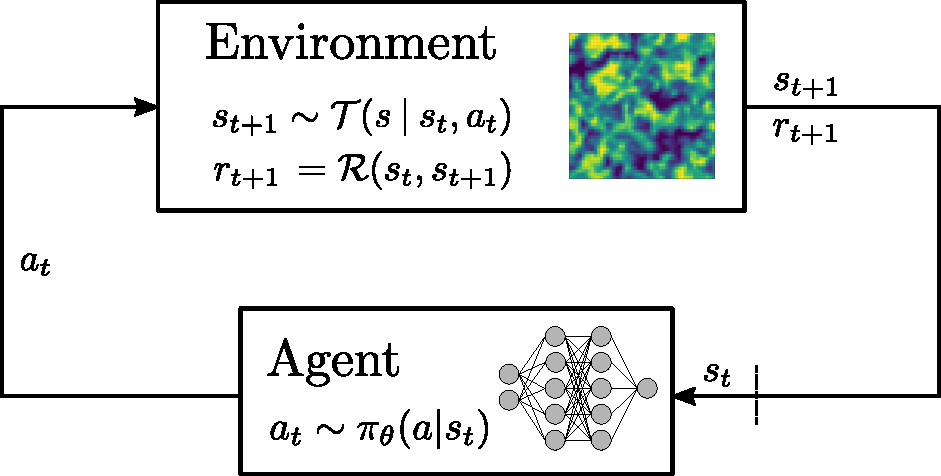
\includegraphics[width=0.7\linewidth]{RL_MDP.pdf}
  \caption{Schematic of the Markov decision process. The agent performs an action $a_t$ based on its policy $\sgeneralpolicy$ to interact with the environment. Consequently, the environment transitions into a new state $\state_{t+1}$ according to its transition function $\sgeneraltransition$. The resulting reward $\reward_{t+1}$ is specified by the reward function \mbox{$r_{t+1}=\rewardfunc\left(s_t,\state_{t+1}\right)$}, which is used to quantify how desirable a given state transition is. Starting from an initial environment state $\state_0$ this process is repeated until a final state $\state_n$ is reached. }
  \label{fig:MDP}
\end{figure}


In contrast to the supervised learning approach, reinforcement learning trains an agent by letting it interact with a dynamical environment in order to achieve a pre-defined goal.
This has the advantage that the dynamics of the environment are incorporated into the training process directly by design.
The interplay of the agent and the environment can be framed as a Markov decision process (MDP), as illustrated in \figref{fig:MDP}.
In a MDP, the environment is characterized by its current state $s_t\in\states$.
The agent observes that state and can perform a suitable action $a_t\in\actions$.
Here, $\states$ is the set of all possible environment states and $\actions$ is the set of all possible actions that can be performed by the agent.
The agent's actions are determined by its policy $\sgeneralpolicy$ that states which action the agent should perform given the environment's current state $\state_t$.%
\footnote{
  To keep the notation short, we use the abbreviated notation of $\sgeneralpolicy$ for $\policy_{\modelparam}(\action\sgiven\state=\state_{t})$ which describes the conditional probability of choosing action $\action$ given the current state $\state_t$.
The same holds for the transition function $\transition\left(\state'\sgiven\state=\state_{t},\action=\action_{t}\right)$, which will be abbreviated as $\sgeneraltransition$.
}.
The policy can be of any functional form, but for deep RL, the policy is typically an ANN with parameters $\modelparam$.
The agent's action causes the environment to change is state.
This new state is prescribed by the environment's transition function $\state_{t+1}\sample\sgeneraltransition$, which thus encodes the environment's dynamics.
With the state transition, the agent receives a reward $\reward_{t+1}$ that is determined by the reward function $\reward_{t+1}=\rewardfunc(\state_{t},\state_{t+1})$ and quantifies how desirable a certain state transition is.
The new state $s_{t+1}$ is then again observed by the agent, which performs another action $a_{t+1}$ as prescribed by its current policy.
Starting from some initial state $\state_0$ and performing actions until a final state $\state_n$, this results in a trajectory of states, actions and rewards termed an episode:
\begin{equation}
  \traj = \left\{ \left(\state_0,\action_0,\reward_1\right),\left(\state_1,\action_1,\reward_2\right),\:......\;,\left(\state_{n-1},\action_{n-1},\reward_{n}\right),\state_n\right\} \eqnperiod
  \label{eq:trajectory4}
\end{equation}
The goal of an RL algorithm is to establish an optimization problem that allows to find the optimal policy $\policy^{\opt}$, which maximizes the expected return along an episode
\begin{equation}
  \return(\tau) = \sum_{t=1}^{n} \discount^t r_{t} \eqnperiod
\end{equation}
Here, $\discount$ denotes the discount factor that can be used to balance the importance of short-term and long-term rewards.
In deep RL, finding the optimal policy is equivalent to finding the set of optimal model parameters $\modelparam^{\opt}$ for the employed ANN.

For each state $\state$, the \textit{state-value function} describes the total return which can be expected starting from state $\state_t$ and following a specific policy $\policy$ from there on.
This state-value function can thus be written as
\begin{equation}
  \valuefunction^\policy \left(\state\right) = \expectation\left[\sum_{k=0}^\infty \discount^k r_{t+k}\given\state_t=\state\right] \eqnperiod
  \label{eq:valuefunction}
\end{equation}
Similarly, an \textit{action-value function} or \textit{Q-function} can be determined, which gives the expected return when starting from state $\state_t$ performing action $\action_t$ and following the policy $\policy$ from there on, which reads
\begin{equation}
  \qfunction^\policy \left(\state,\action\right) = \expectation\left[\sum_{k=0}^\infty \discount^k r_{t+k}\given\state_t=\state, \action_t=\action\right] \eqnperiod
  \label{eq:qfunction}
\end{equation}
Based on \eqref{eq:valuefunction} and \eqref{eq:qfunction}, one can define the \textit{advantage function}
\begin{equation}
  \ppoadvantage^\policy \left(\state,\action\right) =  \qfunction^\policy \left(\state,\action\right) - \valuefunction^\policy \left(\state\right) \eqncomma
  \label{eq:advantagefunction}
\end{equation}
which quantifies whether taking action $a_t$ in state $s_t$ increases or decreases the expected return in comparison to performing the action prescribed by the current policy.

Solving a given problem with RL thus requires that the problem is casted into an MDP by a domain expert, i.e. defining the environment's possible states $\states$, its transition function $\sgeneraltransition$, the agent's action space $\actions$, the reward function $\rewardfunc(s_t,s_{t+1})$ and, finally, the ANN architecture used for the policy $\sgeneralpolicy$.
With these definitions in place, a suitable RL algorithm can be applied to find a favorable policy.
Each distinct RL algorithm prescribes how interactions of the agent and the environment are collected and how this sampled experience can be used to optimize the policy such that the expected future return is increased.
RL algorithms differ for instance in terms of sample efficiency and whether they allow for continuous state and action spaces.
In the following, we use proximal policy optimization (PPO) as our RL algorithm of choice, which belongs to the class of policy gradient methods.





\subsection{Policy Gradient Methods}
\label{sec:vpg}


The key idea of policy gradient methods is to optimize the policy directly instead of learning the Q-function in \eqref{eq:qfunction} and inferring the policy implicitly from it.
To this end, policy gradient methods derive a gradient estimator that gives the direction in which the model parameters $\modelparam$ have to be changed in order to increase the expected return.
Given this gradient, the model parameters can be updated with a suitable gradient-ascent algorithm.
Following the \textit{policy gradient theorem}, see e.g. \cite{sutton2018reinforcement}, the gradient estimator can be written as
\begin{equation}
  \policygradient = \expectation\Big[\qfunction^{\policy}\left(\state,\action\right) \,\nabla_{\modelparam}\log \policy_{\modelparam}\left(\action\sgiven\state \right) \Big],
  \label{eq:pg_gradient}
\end{equation}
and can be obtained by differentiating the corresponding loss function
\begin{equation}
  \loss^{VPG}(\modelparam) = \expectation\Big[ \qfunction^{\policy}\left(\state,\action\right) \,  \log \policy_{\modelparam}\left(\action\sgiven\state \right)\Big],
  \label{eq:pg_loss}
\end{equation}
with respect to $\modelparam$.
Since the policy and the environment are in general stochastic, the gradient estimator for the optimization is defined by means of the expectation $\expectation\left[\cdot\right]$.
However, obtaining the exact expectation is prohibitive for practical applications.
Instead, the gradient estimator is approximated by sampling $N$ trajectories of experience on the current policy and computing the approximated gradient as mean over the sampled trajectories
\begin{equation}
  \hat{\policygradient} = \frac{1}{N}\sum_{i=1}^N\left[\return\left(\traj^{(i)}\right) \ \sum_{t=0}^n  \nabla_{\modelparam}\log \policy_{\modelparam}\left(\action_t\sgiven\state_t \right)\right] \eqnperiod
  \label{eq:pg_approx_gradient}
\end{equation}
Here, the discounted return along a trajectory $\return(\traj)$ is used as an approximation to the exact Q-function.
Interestingly, the dynamics of the environment, i.e. its transition function $\sgeneraltransition$, do not appear in the gradient estimator or in the overall optimization formulation.
Instead, the dynamics of the environment are incorporated implicitly by the sampled experience.
This avoids to differentiate the environment dynamics with respect to the policy parameters, which is infeasible for most tasks.

The training process of a policy gradient method then works as follows.
First, multiple episodes of experience are sampled with the current policy.
Based on this experience, the policy can be optimized in a second step with the gradient estimator and a suitable gradient-ascent algorithm.
These two steps are then repeated, until the policy has converged.
These building blocks form the vanilla policy gradient (VPG) method.

\subsection{Proximal Policy Optimization}
\label{sec:ppo}

The proximal policy optimization (PPO) method \cite{schulman2017proximal} introduces several improvements over the original vanilla policy gradient (VPG) method to improve the stability of the training.
For a clear and concise summary of the PPO algorithm, we recommend \cite{notter2021hierarchical}.

The first major improvement of PPO is to reduce the variance of the gradient estimator.
This reduces the amount of samples required for an accurate approximation of the gradient or a better gradient estimator for a given amount of samples.
To this end, a baseline can be added to the gradient estimator in \eqref{eq:pg_approx_gradient}, which has been shown to not introduce a bias.
A natural choice is to replace the Q-function by the advantage function from \eqref{eq:advantagefunction}.
However, the advantage function relies on the state-value function $\valuefunction^{\policy}(s)$, which is typically unknown.
Therefore, the PPO algorithm uses an additional ANN $\hat{\valuefunction}_{\valueparam}(s)$ with weights $\valueparam$, which is trained to approximate the state-value function.
Moreover, the return along the trajectory, which approximates the Q-function, is replaced by a \textit{return-to-go} $R_t(\tau) = \sum_{k=t}^n \gamma^{k-t} r_k$ such that each action is only associated with reward that is collected after the action is taken.
The approximate advantage function at step $t$ thus reads
\begin{equation}
  \hat{\ppoadvantage}_t = \left(\sum_{k=t}^n \gamma^{k-t} r_k\right) - \hat{\valuefunction}_{\valueparam}(s_t).
  \label{eq:ppo_advantage}
\end{equation}

A major drawback of VPG is that the training with the VPG method is often found to be unstable, since the policy updates can become arbitrarily large.
Large policy updates imply the risk of deteriorating the policy's performance in a single update step if the gradient estimator is not sufficiently accurate or the step size is too large.
The PPO method increases the stability of the training process by constraining the maximum change of the policy in a single step. %
Schulman et al. \cite{schulman2017proximal} propose two different approaches to limit the updates of the policy.
Firstly, a penalty term can be added to \eqref{eq:pg_loss} based on the Kullback-Leibler divergence between the old and the new policy.
This introduces the incentive to avoid large changes in the policy in a single training step.
The other approach is to replace the loss function in \eqref{eq:pg_loss} by a clipped surrogate objective
\begin{equation}
  \loss^{CLIP}(\modelparam) = \expectation\left[\min\left( \probratio\left(\modelparam\right)\hat{\ppoadvantage},\mathrm{clip}\left(\probratio\left(\modelparam\right),1-\eps,1+\eps\right)\hat{\ppoadvantage}   \right)   \right],
  \label{eq:clipping_loss}
\end{equation}
with $\eps$ as a hyperparameter and with $\probratio(\modelparam)$ as the probability ratio
\begin{equation}
  \probratio\left(\modelparam\right)=\frac{\policy_{\modelparam}\left(\action\sgiven\state\right)}{\policy_{\modelparam_{old}}\left(\action\sgiven\state\right)},
  \label{eq:prob_ratio}
\end{equation}
which describes the change between the old and the new policy.
In \eqref{eq:clipping_loss}, the clip function clips the probability ratio $\probratio(\modelparam)$ to the interval $\left[1-\epsilon,1+\epsilon\right]$ to limit the change of the policy in a single training step.
Similarly to \eqref{eq:pg_approx_gradient}, the expectation in \eqref{eq:clipping_loss} is then approximated by sampling trajectories with the current policy.

